

\documentclass{beamer}
 
\usepackage[utf8]{inputenc}
 
 
%Information to be included in the title page:
\title{JEE problem in python}
\author{}{}
\author{
  Akhil George Thomas : CS17BTECH11047
  \and \newline
  Vijay Tadikamalla : CS17BTECH11040
}
\institute{IITH}
\date{12th February, 2019}
 
 
 
\begin{document}
 
\frame{\titlepage}
\begin{frame}
\frametitle{The question}
A hyperbola passes through the point 
\begin{equation}
\vec{P}=(\myvec{\sqrt{2}, \sqrt{3}})
\end{equation}
and has foci at $(\myvec{\pm 2, 0})$.  Find the equation of the tangent to this hyperbola at 
$\vec{P}$.
\end{frame}

\begin{frame}
\frametitle{Approach}
We know the distance between the two foci is $2ae$.
\pause
\bigbreak
We know that the difference between the distances from a point on the hyperbola to the two foci is a constant.
\pause
\bigbreak

This constant is equal to $2a$.
\pause
\bigbreak
We also know that, 

\centering
$b^2 = a^2*(e^2-1)$
\end{frame}
\begin{frame}
\frametitle{Approach}
Each point is represented as an numpy array.
\bigbreak
A hyperbola of the form

\begin{center}
$\frac{x^2}{a^2} - \frac{y^2}{b^2} = 1$ 
\end{center}

in matrix form is represented as:

\begin{center}
$ x^T * V * x = c$
\end{center}


which is same as:
\[
\begin{bmatrix}
    x & y
\end{bmatrix}
\begin{bmatrix}
    1/a^2  &  0      \\
    0  &  -1/b^2      
\end{bmatrix}
\begin{bmatrix}
    x       \\
    y
\end{bmatrix}
= 
\begin{bmatrix}
    1      
\end{bmatrix} 
\]
\end{frame}
\begin{frame}
\frametitle{Approach}
The hyperbola is:
\[
\begin{bmatrix}
    x & y
\end{bmatrix}
\begin{bmatrix}
    1/a^2  &  0      \\
    0  &  -1/b^2      
\end{bmatrix}
\begin{bmatrix}
    x       \\
    y
\end{bmatrix}
= 
\begin{bmatrix}
    1      
\end{bmatrix} 
\]
And the point form of tangent at point $P (x_1,y_1)$ for the above hyperbola is:
\[
\begin{bmatrix}
    x & y
\end{bmatrix}
\begin{bmatrix}
    1/a^2  &  0      \\
    0  &  -1/b^2      
\end{bmatrix}
\begin{bmatrix}
    x_1       \\
    y_1
\end{bmatrix}
= 
\begin{bmatrix}
    1      
\end{bmatrix} 
\]
\end{frame}

\begin{frame}
\frametitle{Graphical Verification}
\begin{figure}[H]
\centering
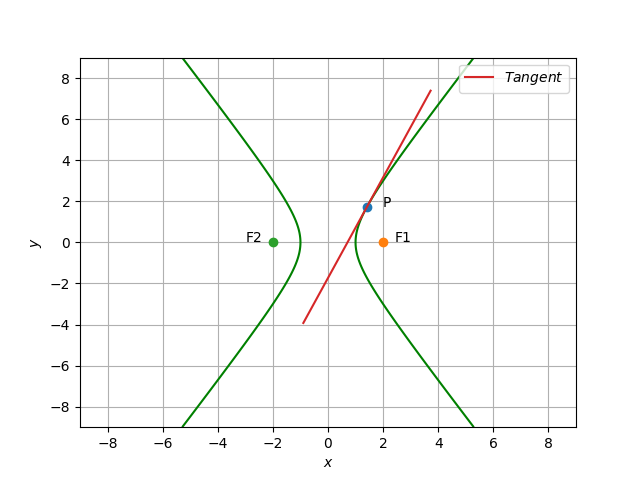
\includegraphics[scale=0.5]{hyperbola_img.png}
\end{figure}
\end{frame}
\end{document}

